\section{Schematy warstwy danych}

	\subsection{Schemat tabel}
	Diagramy poniżej przedstawiają schemat bazy danych. Dla większej czytelności zostały one podzielone na mniejsze rysunki.
	Każdy z nich przedstawia logicznie powiązane ze sobą tabele. 
	\begin{figure}[th]
		\centering
		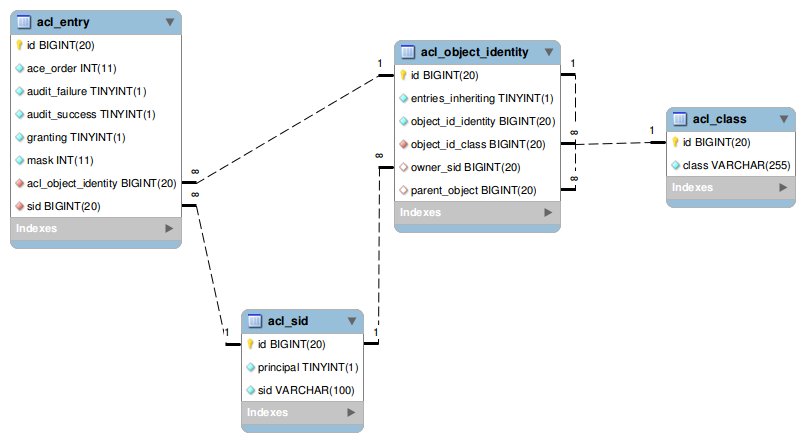
\includegraphics[width=1.0\textwidth]{images/db/acl}
		\caption[Tabele grupy \textit{acl}]{
			Tabele grupy \textit{acl}
		}
		\label{app:schema_db}
	\end{figure}
	\clearpage
	\begin{figure}[H]
		\centering
		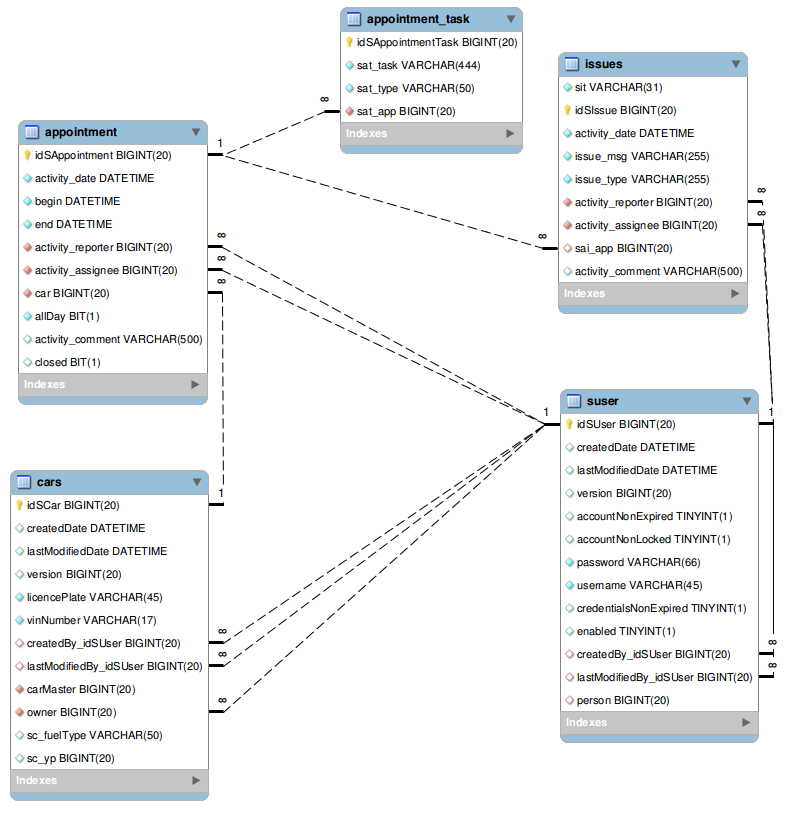
\includegraphics[width=1.0\textwidth]{images/db/appointment}
		\caption[Tabele grupy \textit{appointment}]{
			Tabele grupy \textit{appointment}
		}
		\label{app:schema_db}
	\end{figure}
	\begin{figure}[H]
		\centering
		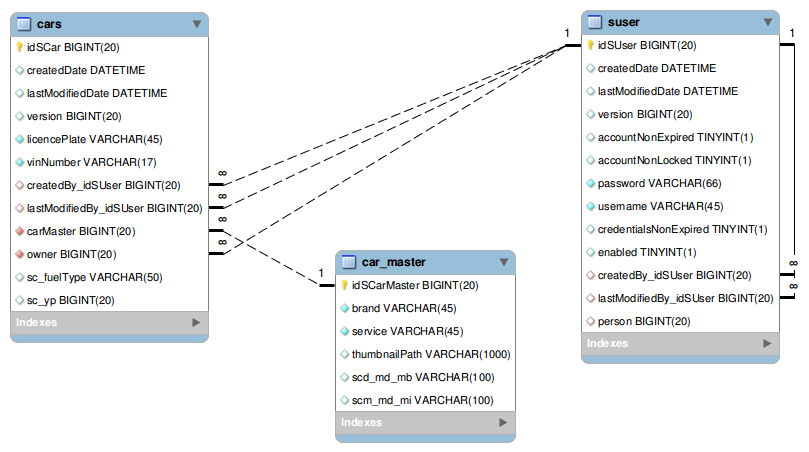
\includegraphics[width=1.0\textwidth]{images/db/car}
		\caption[Tabele grupy \textit{car}]{
			Tabele grupy \textit{car}
		}
		\label{app:schema_db}
	\end{figure}
	\begin{figure}[H]
		\centering
		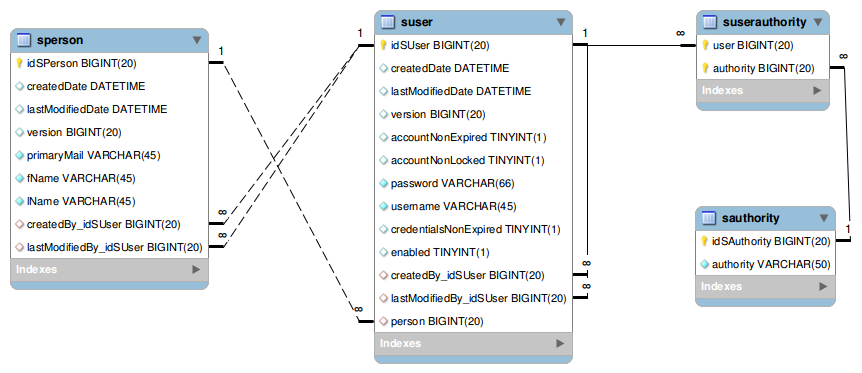
\includegraphics[width=1.0\textwidth]{images/db/user}
		\caption[Tabele grupy \textit{user}]{
			Tabele grupy \textit{user}
		}
		\label{app:schema_db}
	\end{figure}
	\begin{figure}[H]
		\centering
		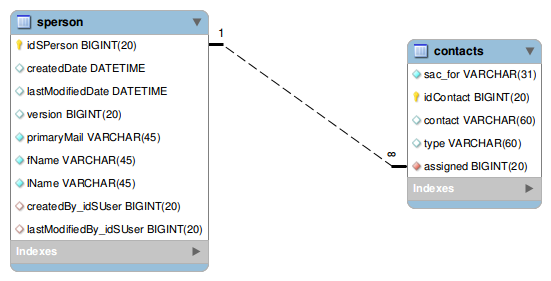
\includegraphics[width=1.0\textwidth]{images/db/person}
		\caption[Tabele grupy \textit{person}]{
			Tabele grupy \textit{person}
		}
		\label{app:schema_db}
	\end{figure}
	\begin{figure}[H]
		\centering
		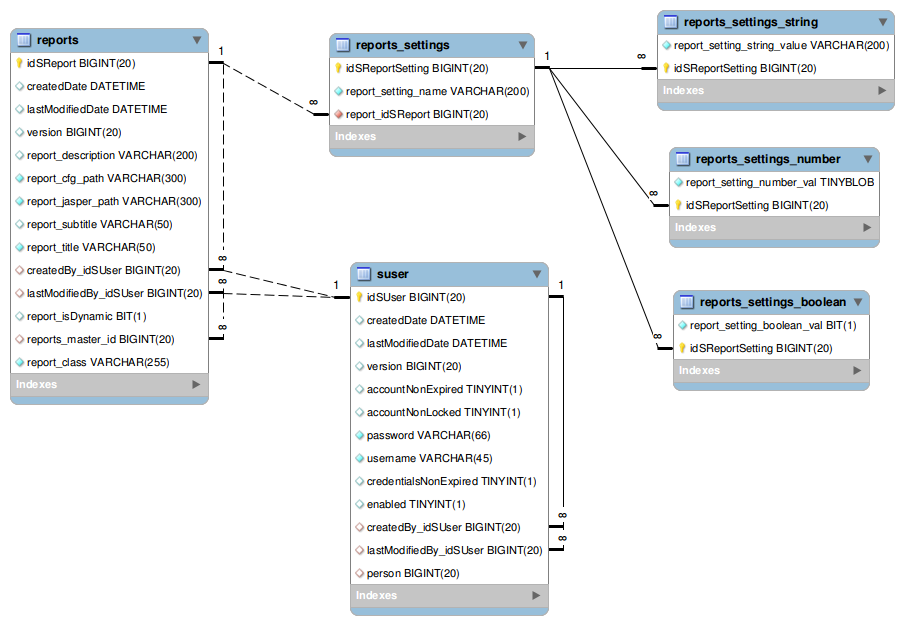
\includegraphics[width=1.0\textwidth]{images/db/report}
		\caption[Tabele grupy \textit{report}]{
			Tabele grupy \textit{report}
		}
		\label{app:schema_db}
	\end{figure}
	\begin{figure}[H]
		\centering
		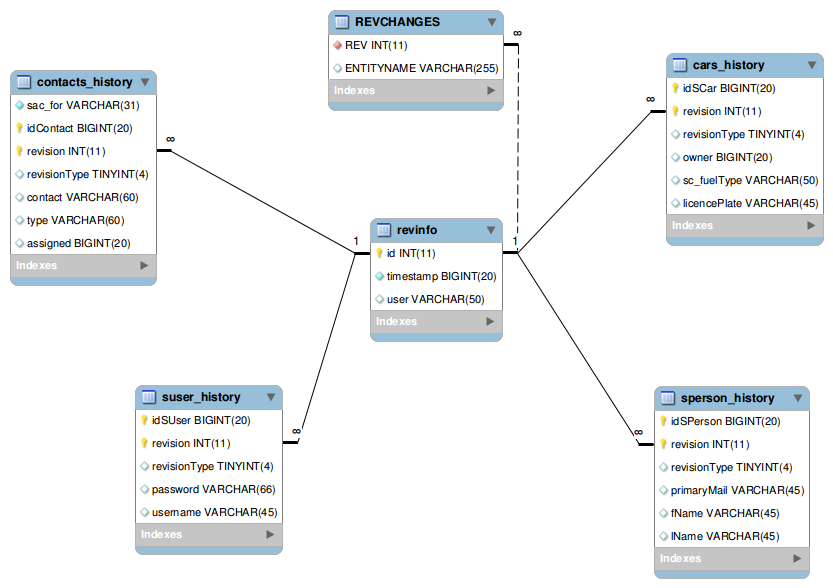
\includegraphics[width=1.0\textwidth]{images/db/history}
		\caption[Tabele grupy \textit{history}]{
			Tabele grupy \textit{history}
		}
		\label{app:schema_db}
	\end{figure}
	
	\clearpage
	\subsection{Schemat obiektowy}
	Poniższe rysunki przedstawiają diagramy klas poszczególnych paczek opisujących model danych. 
	Na wszystkich diagramach pominięte zostały metody dostępowe (gettery oraz settery). 
	
	\begin{figure}[H]
		\centering
		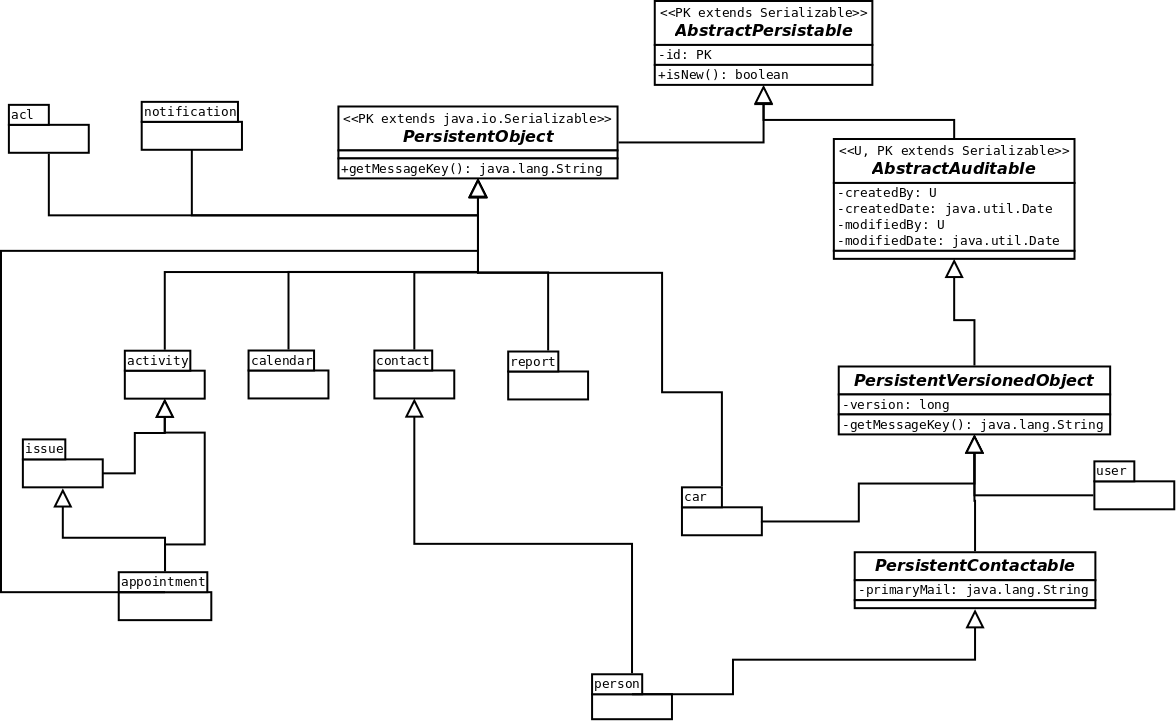
\includegraphics[width=1.0\textwidth]{images/umls/object_model}
		\caption[Obiektowy model danych]{
			Obiektowy model danych
		}
		\label{app:schema_org_agatom_springatom_model} 
	\end{figure}
	\begin{figure}[H]
		\centering
		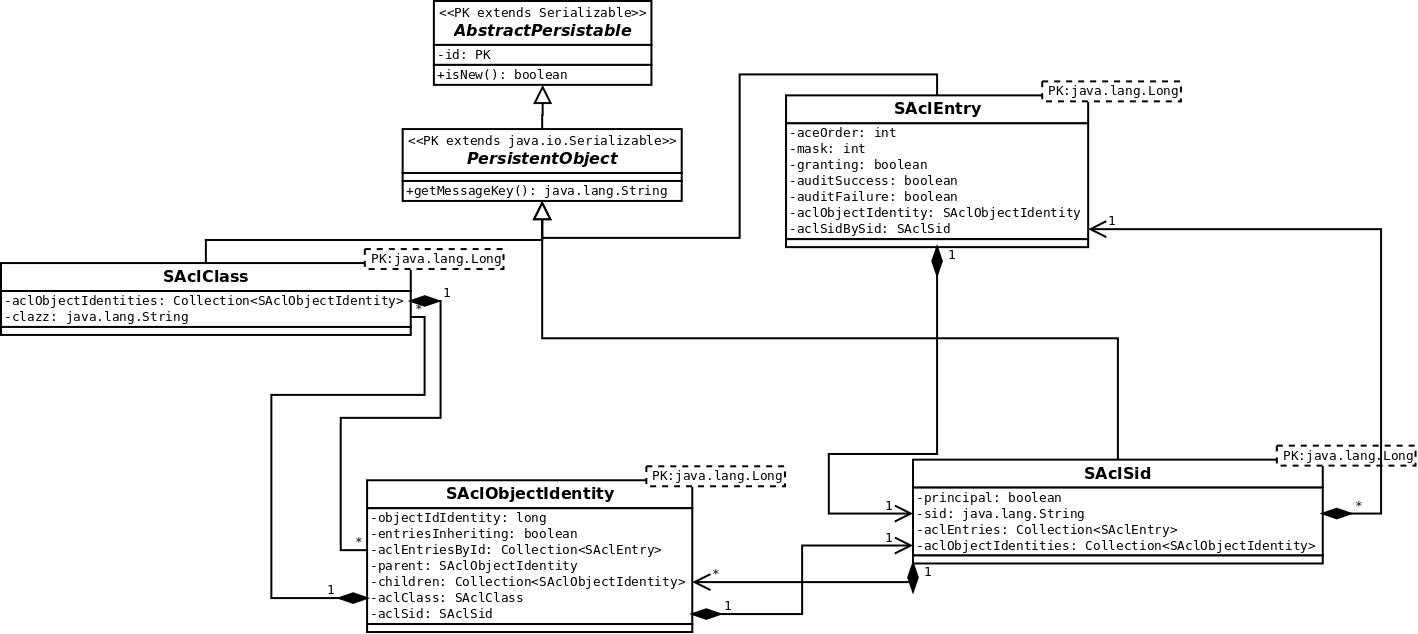
\includegraphics[width=1.0\textwidth]{images/umls/acl}
		\caption[Obiektowy model danych - Paczka \textbf{acl}]{
			Obiektowy model danych - Paczka \textbf{acl}
		}
		\label{app:schema_acl_package}
	\end{figure}
	\begin{figure}[H]
		\centering
		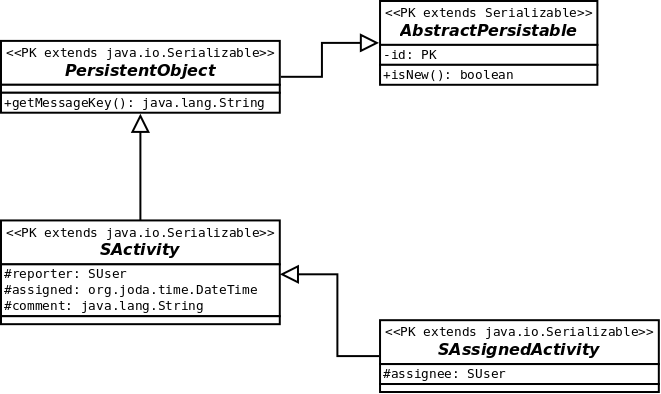
\includegraphics[width=0.9\textwidth]{images/umls/activity}
		\caption[Obiektowy model danych - Paczka \textbf{activity}]{
			Obiektowy model danych - Paczka \textbf{activity}
		}
		\label{app:schema_activity_package}
	\end{figure}
	\begin{figure}[H]
		\centering
		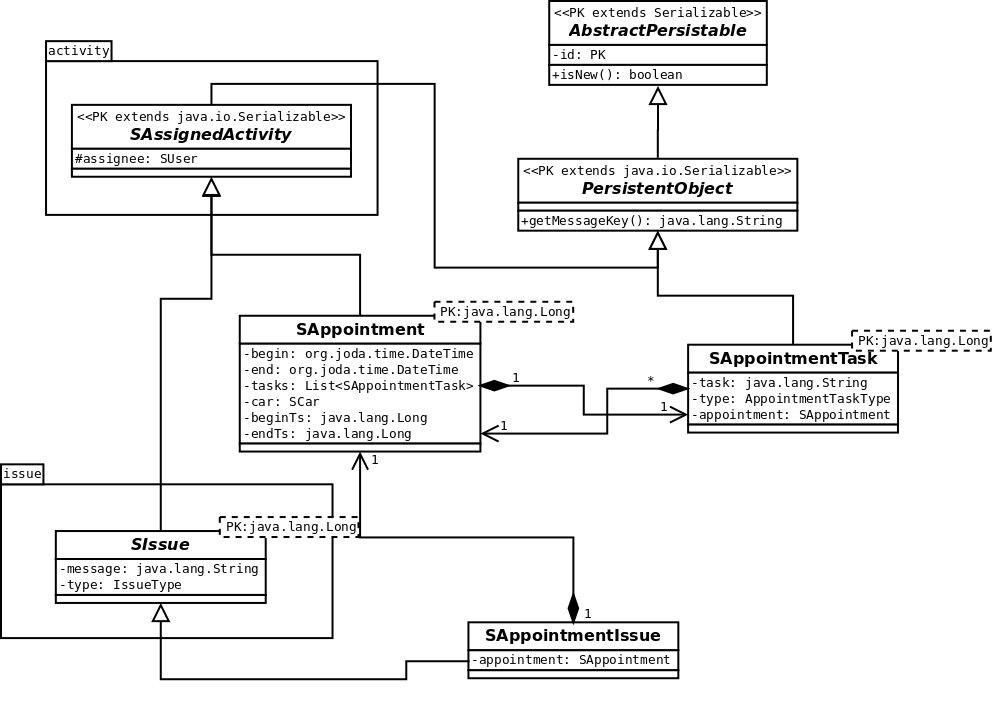
\includegraphics[width=0.9\textwidth]{images/umls/appointment}
		\caption[Obiektowy model danych - Paczka \textbf{appointment}]{
			Obiektowy model danych - Paczka \textbf{appointment}
		}
		\label{app:schema_appointment_package}
	\end{figure}
	\begin{figure}[H]
		\centering
		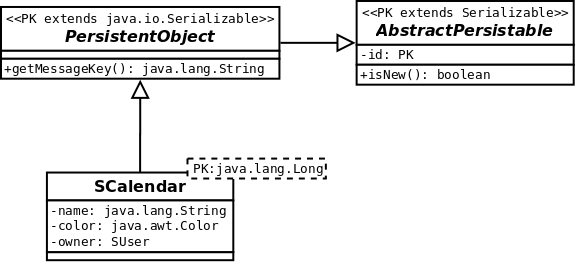
\includegraphics[width=1.0\textwidth]{images/umls/calendar}
		\caption[Obiektowy model danych - Paczka \textbf{calendar}]{
			Obiektowy model danych - Paczka \textbf{calendar}
		}
		\label{app:schema_calendar_package}
	\end{figure}
	\begin{figure}[H]
		\centering
		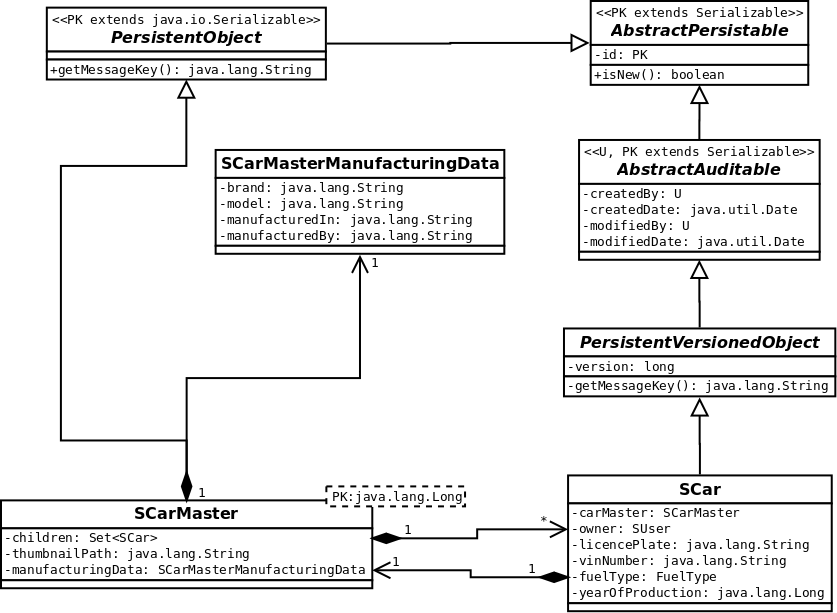
\includegraphics[width=1.0\textwidth]{images/umls/car}
		\caption[Obiektowy model danych - Paczka \textbf{car}]{
			Obiektowy model danych - Paczka \textbf{car}
		}
		\label{app:schema_car_package}
	\end{figure}
	\begin{figure}[H]
		\centering
		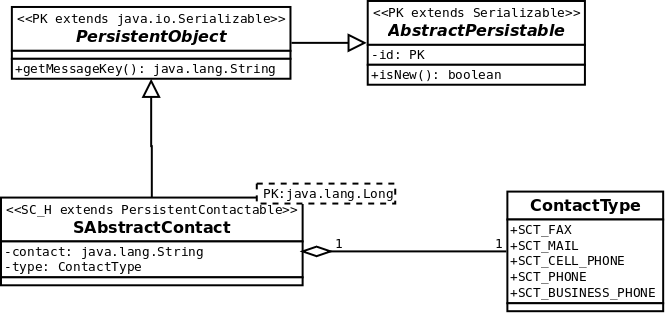
\includegraphics[width=1.0\textwidth]{images/umls/contact}
		\caption[Obiektowy model danych - Paczka \textbf{contact}]{
			Obiektowy model danych - Paczka \textbf{contact}
		}
		\label{app:schema_contact_package}
	\end{figure}
	\begin{figure}[H]
		\centering
		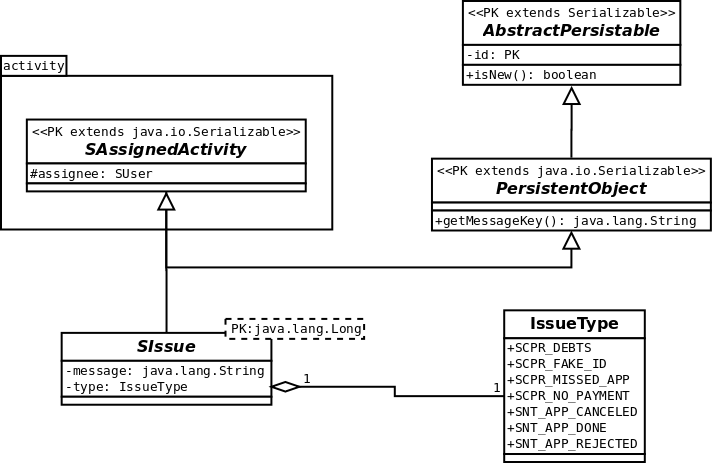
\includegraphics[width=1.0\textwidth]{images/umls/issue}
		\caption[Obiektowy model danych - Paczka \textbf{issue}]{
			Obiektowy model danych - Paczka \textbf{issue}
		}
		\label{app:schema_issue_package}
	\end{figure}
	\begin{figure}[H]
		\centering
		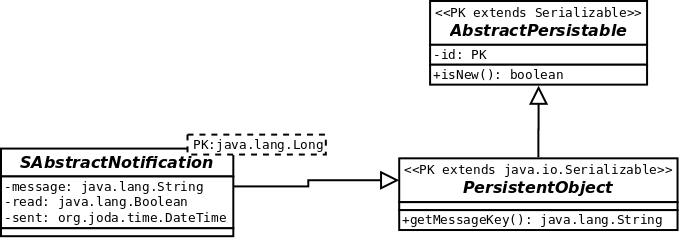
\includegraphics[width=1.0\textwidth]{images/umls/notifications}
		\caption[Obiektowy model danych - Paczka \textbf{notifications}]{
			Obiektowy model danych - Paczka \textbf{notifications}
		}
		\label{app:schema_notifications_package}
	\end{figure}
	\begin{figure}[H]
		\centering
		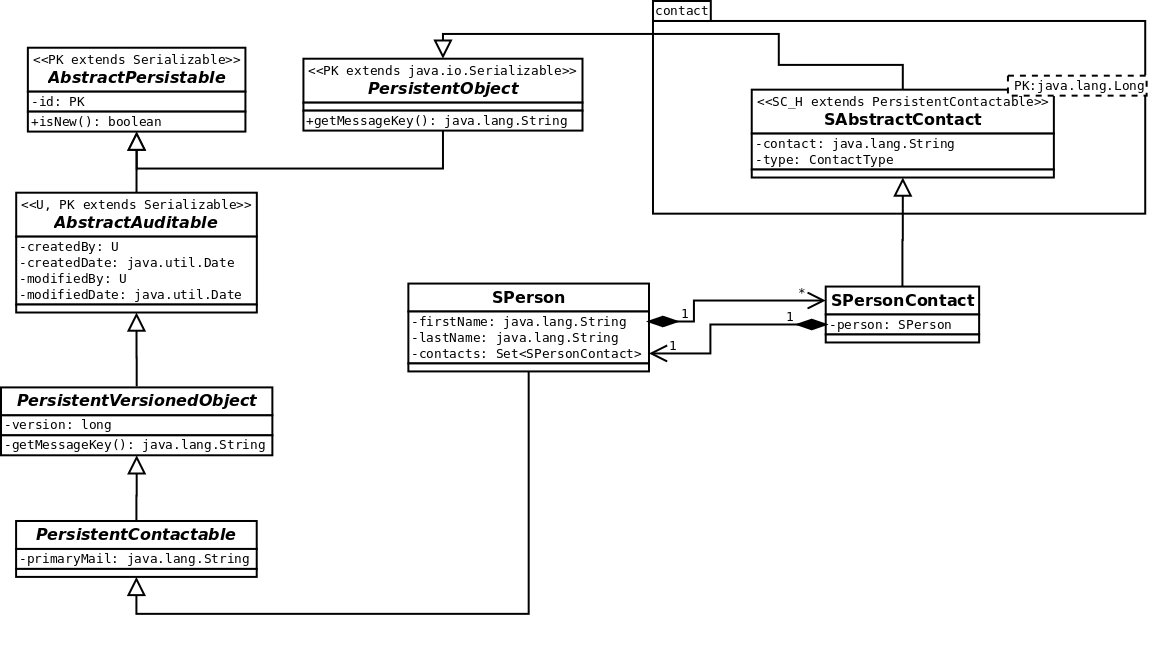
\includegraphics[width=1.0\textwidth]{images/umls/person}
		\caption[Obiektowy model danych - Paczka \textbf{person}]{
			Obiektowy model danych - Paczka \textbf{person}
		}
		\label{app:schema_person_package}
	\end{figure}
	\begin{figure}[H]
		\centering
		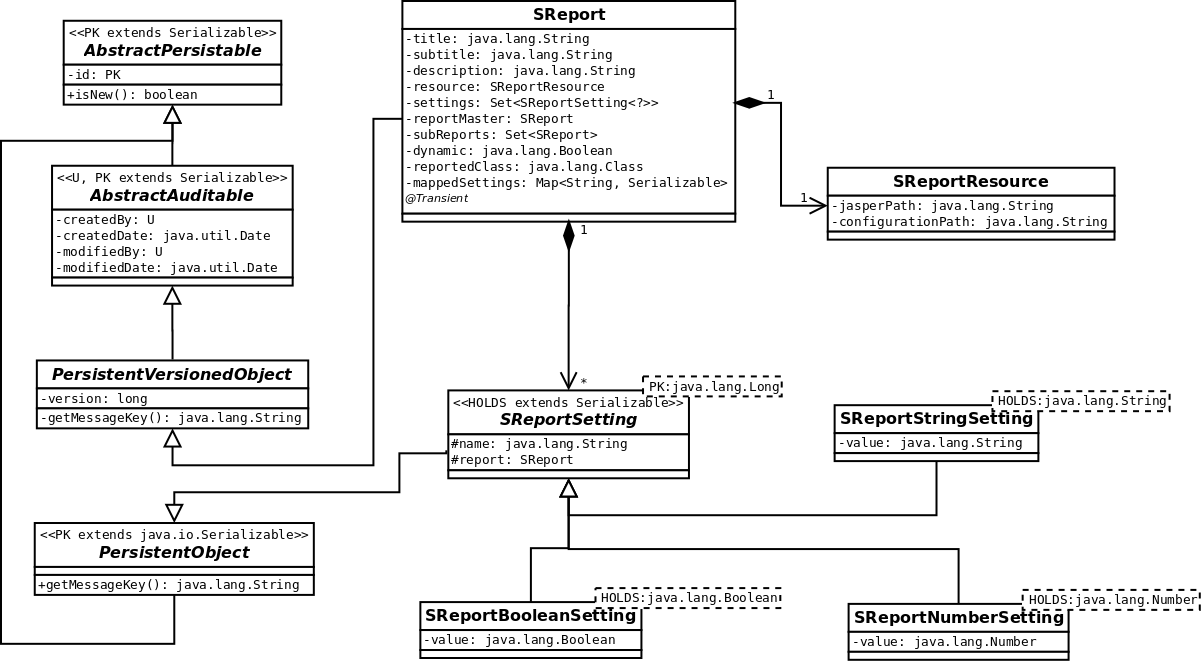
\includegraphics[width=0.9\textwidth]{images/umls/report}
		\caption[Obiektowy model danych - Paczka \textbf{report}]{
			Obiektowy model danych - Paczka \textbf{report}
		}
		\label{app:schema_person_package}
	\end{figure}
	\begin{figure}[H]
		\centering
		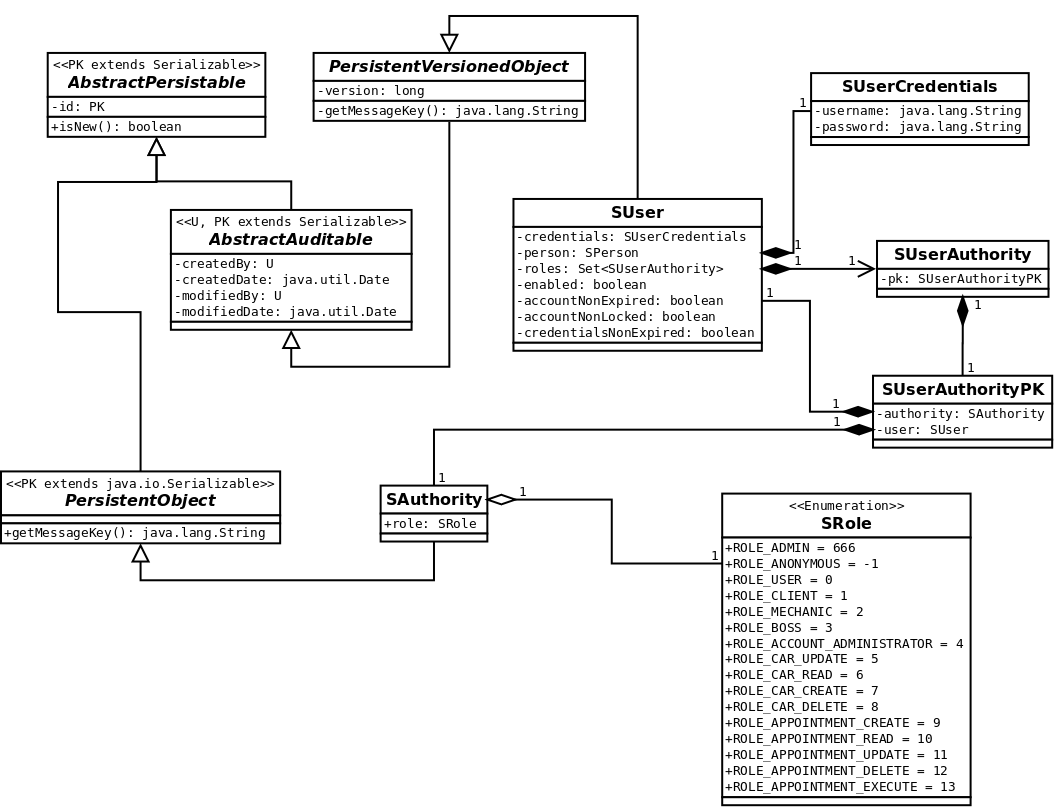
\includegraphics[width=0.9\textwidth]{images/umls/user}
		\caption[Obiektowy model danych - Paczka \textbf{user}]{
			Obiektowy model danych - Paczka \textbf{user}
		}
		\label{app:schema_person_package}
	\end{figure}

\section{Model danych komponentów InfoPage oraz TableComponent}
	\begin{figure}[th]
		\centering
		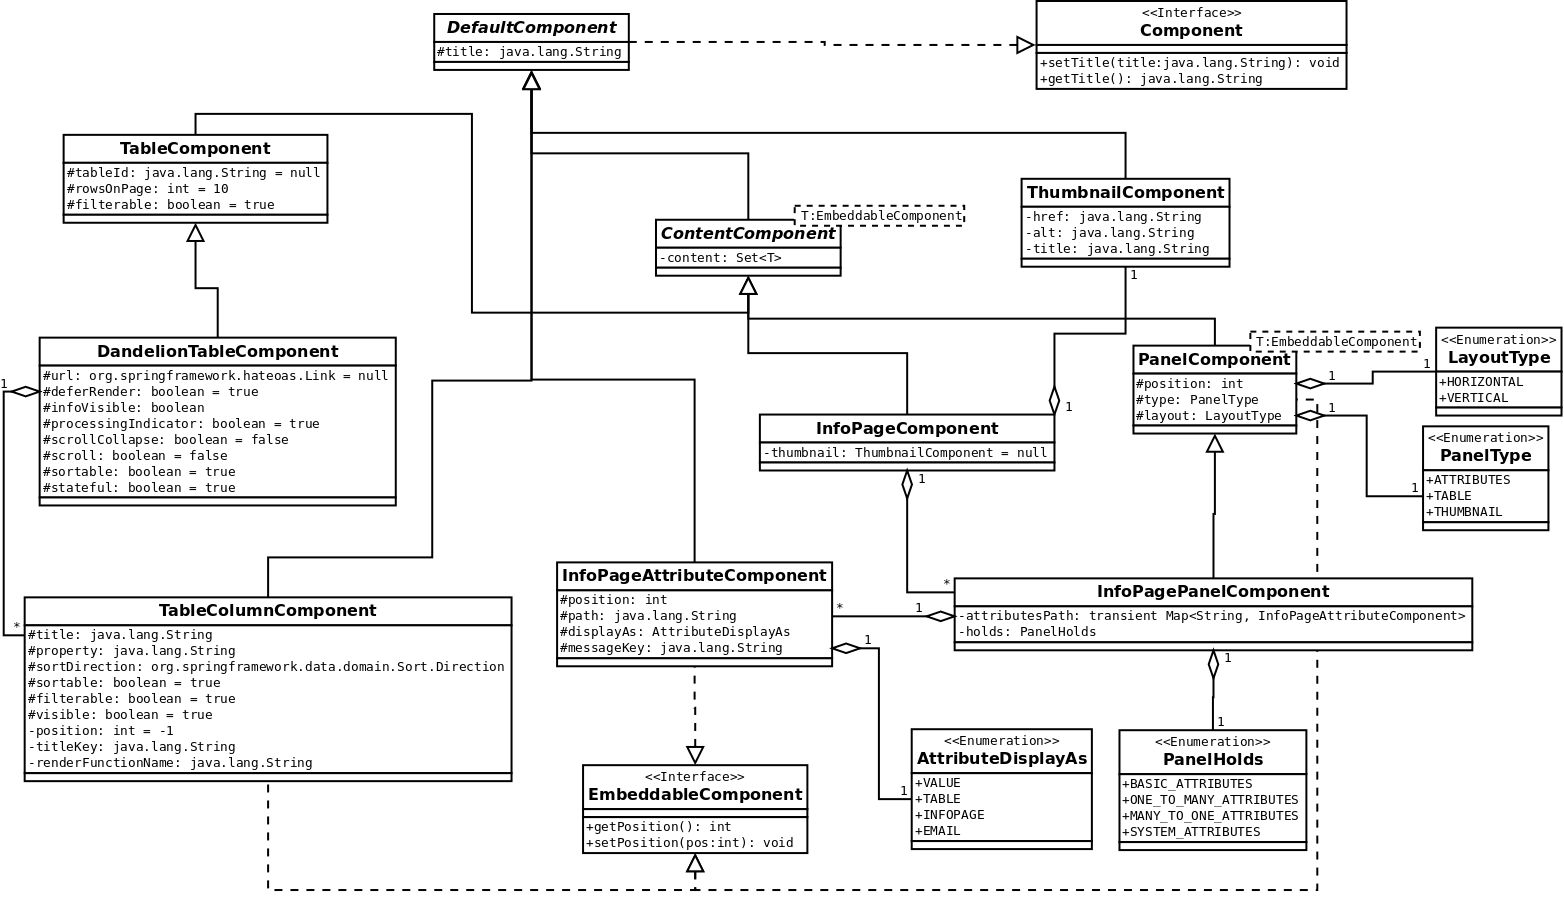
\includegraphics[width=1.0\textwidth]{images/umls/components}
		\caption[Diagram modelu danych komponentów \textbf{InfoPage} oraz \textbf{TableBuilder}]{
			Diagram modelu danych komponentów \textbf{InfoPage} oraz \textbf{TableBuilder}
		}
		\label{app:rbuilder_data_Model}
	\end{figure}

\section{Model danych komponentu \textbf{RBuilder}}
	\begin{figure}[th]
		\centering
		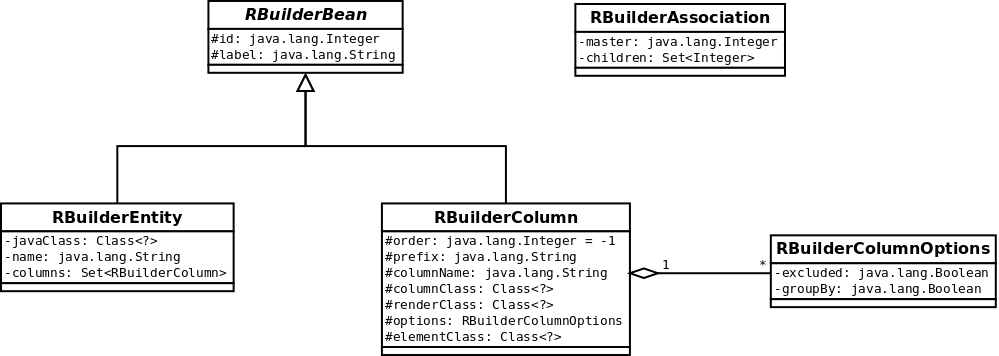
\includegraphics[width=1.0\textwidth]{images/umls/rbuilder}
		\caption[Diagram UML modelu danych \textbf{RBuilder}]{
			Diagram UML modelu danych \textbf{RBuilder}
		}
		\label{app:rbuilder_data_Model}
	\end{figure}
	
